
\newpage
%%%%%%%%%%%%%%%%%%%%%%%%%%%%%%%%%%%%%%%%%%%%%%%%%%%%%%%%%%%%%%%%%%%%%%%%%%%%%%%%
%%%%%%%%%%%%%%%%%%%%%%%%%%%%%%%%%%%%%%%%%%%%%%%%%%%%%%%%%%%%%%%%%%%%%%%%%%%%%%%%
\section{Dançar no ritmo}
\label{subsec:dancaritmo}
\index{Musicalidade!Dançar no ritmo}
 Dançar usando o \hyperref[sec:pos:Ritmo]{\textbf{ritmo}},
é um estágio intermediário de nosso percorrido para melhorar nossa musicalidade;
para atingir a competência neste estagio, 
primeiro devemos ter dominado \hyperref[subsec:dancametrica]{\textbf{dançar na métrica}},
para logo aprender a aproveitar as informações encontradas 
no ritmo que não foram aproveitadas quando estudamos dançar na métrica. 

O ritmo pode vir da parte rítmica de uma melodia, 
algum acompanhamento percussivo ou harmônico, 
ou da convergência de todos os instrumentos na música.
No modo mais cru, poderíamos pensar no ritmo
como um conjunto de \hyperref[sec:figurasmusicais]{\textbf{figuras musicais}} 
colocadas uma apos de outra, 
e explorar o ritmo, figura a figura musical. % este \hyperref[sec:elementosmusica]{\textbf{elemento da música}}.
Porem, ao igual que quando escutamos um discurso,
sabemos que este é um conjunto de letras colocadas uma apos outra,
e poderíamos estudar-lho desde essa perspetiva;
para nós seres humanos, 
muitas vezes é mais fácil pensar em ``macro'' que em ``micro'',
ou seja em estruturas maiores como palavras ou frases, perguntas, respostas, etc. 
Donde nosso cérebro, em muitos casos, 
já tem soluciones prontas para atender estes problemas.


Assim, podemos abordar o problema de dançar no ritmo das seguistes formas:
%desde uma perspetiva mais abrangente (macro) ou desde uma perspetiva mais simplista (micro).
\begin{description}
\item [Nível micro:] Para desenvolver este ponto devemos lembrar 
que existem 4 \hyperref[sec:carateristasom]{\textbf{características básicas do som}},
sendo estas: 
\begin{inparaitem}
\item o tom, 
\item a duração, 
\item o timbre e 
\item a intensidade.
\end{inparaitem}
Destas quatro só o tom não vai ser aproveitado quando dançamos no ritmo;
porem, podemos usar o timbre e a intensidade do som para mudar nossas 
\hyperref[sec:musicalidade:dinamicas]{\textbf{dinâmicas do movimento}};
já a duração poderia ser aproveitada dançando figura musical a figura musical,
movimentando-nos atrelados a esse elemento. 


\item [Nível macro:] Neste nível podemos aproveitar os  motivos e frases rítmicas
provenientes de instrumentos de percussão, ou da parte rítmica de uma melodia ou acompanhamento harmônico;
de modo que podemos interpretar estes motivos e frases rítmicas, 
com suas obvias consequências: como o melhor aproveitamento das pausas
 nos finais de frase musical ou nos ``breaks'' da música (ver Exemplo \ref{ex:ritmo:usingbreak}),
ou realizando mudanças de movimentos nas mudanças de frases rítmicas.
Isto é similar ao que faríamos nas frases (melódicas) só que aqui 
não tomamos em conta a informação das mudanças de tom.
\end{description}
%Assim, quando percebemos o ritmo numa música, 
%podemos sim usar este elemento da música, figura a figura; 
%porem, devemos lembrar que temos outros aspectos do ritmo,
%agrupadas em estruturas maiores e menos evidentes que podemos aproveitar.


\begin{example}[Usando a duração das figuras musicais (Nível micro):]
\label{ex:dancaritmo1}
Imaginemos que temos decidido executar nossos movimentos (ex: pisadas, ou movimentos de ombros, cabeça quadril, etc.),
seguindo o ritmo de uma camada numa peça musical.
Neste caso, uma alternativa para dançar no ritmo, 
seria movimentar nosso corpo seguindo uma a uma as figuras musicais;
é dizer, dando um passo ou realizando uma troca de peso somente quando é executada uma figura musical.

Assumindo esta  consideração artística para nossos movimentos, 
podemos usar a parte rítmica da melodia ``Lamento e consolo'', descrita na Figura \ref{fig:lamento-e-consolo},
para dançar no ritmo, 
de modo que nossos movimentos sejam executados como indica a Figura \ref{fig:lamentoconsoloritmo1}.
A melodia está descrita para ser interpretada com um ``bandolim'';
sendo que as ``claves'' na pauta representam o ritmo proposto que devem seguir nossos movimentos;
neste caso foram escolhidos pisadas, como movimentos de exemplo.

Se desejamos treinar dançar no ritmo, só com a base rítmica e sem as mudanças de tom,  
podemos usar a pauta descrita na Figura \ref{fig:lamentoconsoloritmo2} que é uma versão 
reduzida da pauta da Figura \ref{fig:lamentoconsoloritmo1}.

%É fácil perceber, na representação das Figuras \ref{fig:lamentoconsoloritmo1} e \ref{fig:lamentoconsoloritmo2}, 
%que nossos movimentos estão atrelados ao ritmo da melodia,
%e não a outras informações como o tom das notas musicais.
\end{example}
\begin{sidewaysfigure}
    \centering
    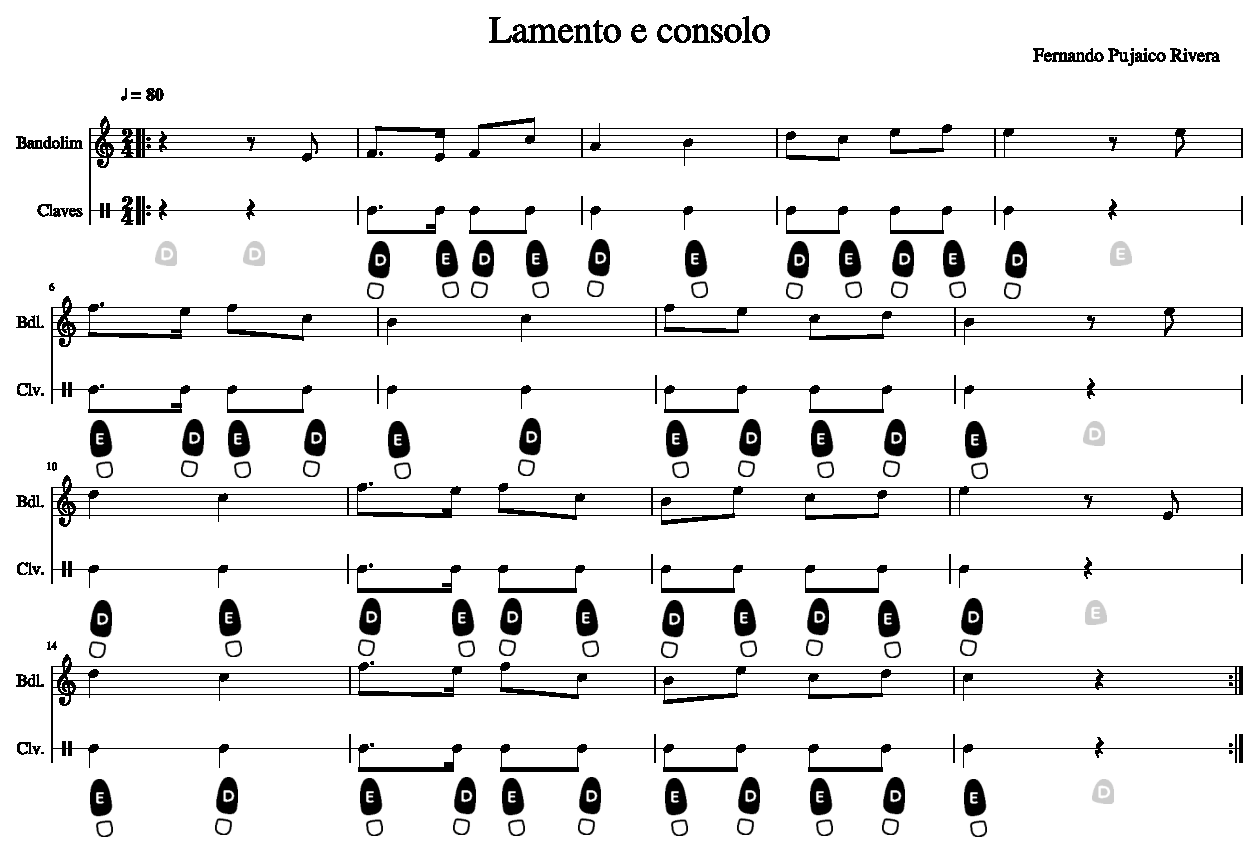
\includegraphics[width=\textwidth]{chapters/cap-musicalidade-tecnica/lamento-e-consolo-clave-ritmo-1.eps}
    \caption{Música dançada no ritmo.}
    \label{fig:lamentoconsoloritmo1}
\end{sidewaysfigure}


\begin{sidewaysfigure}
    \centering
    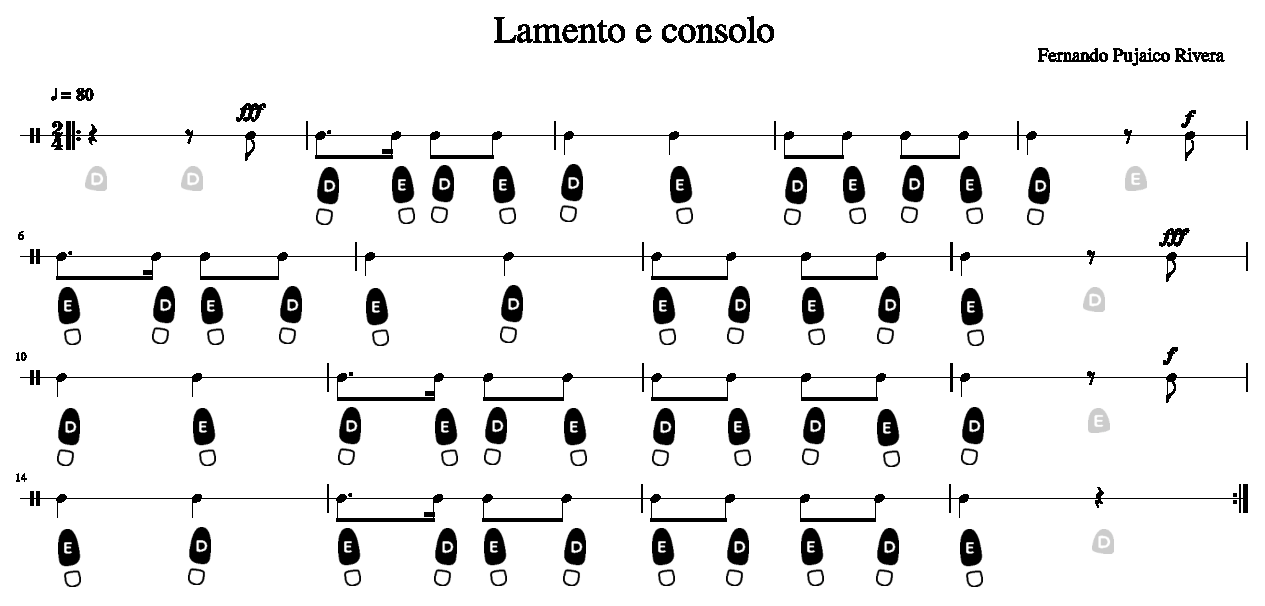
\includegraphics[width=\textwidth]{chapters/cap-musicalidade-tecnica/lamento-e-consolo-clave-ritmo2-1.eps}
    \caption{Parte rítmica da melodia ``Lamento e consolo''.}
    \label{fig:lamentoconsoloritmo2}
\end{sidewaysfigure}

\begin{example}[Usando a duração das figuras musicais e as frases rítmicas 
(Nível micro e macro):]
\label{ex:dancaritmo1macro}
Neste caso temos decidido executar dois tipos de movimentos 
(que podem ser: pisadas, ou movimentos de ombros, cabeça quadril, etc.),
seguindo a parte rítmica da melodia ``Lamento e consolo'' como mostrado na Figura \ref{fig:lamentoconsoloritmo2}.
Assim, movimentaremos nosso corpo seguindo uma a uma as figuras musicais, 
de forma similar ao feito no Exemplo \ref{ex:dancaritmo1}; porém, 
agora  agregaremos o detalhe que, além de seguir as figuras musicais,
também mudaremos de movimento em cada mudança de frase rítmica.

Assim, se por exemplo escolhemos como movimentos:
mexer os pés e mexer os ombros; nos movimentaremos numa frase rítmica completa usando só os pés,
e na seguinte frase rítmica deixaremos de mover os pés e 
usaremos agora os ombros para seguir as figuras musicais,
e assim sucessivamente durante as 4 frases rítmicas da pauta. 
\end{example}
\begin{example}[Usando a duração e intensidade das figuras musicais e as frases rítmicas 
(Nível micro e macro):]
\label{ex:dancaritmo2macro}
Este exemplo é similar ao Exemplo \ref{ex:dancaritmo1macro}, 
com a diferença que agora também aproveitaremos as intensidades de execução das figura musicais nas frases rítmicas,
sendo as frases 1ra e a 3ra \hyperref[sec:sinaisintensidade]{\textbf{fortissisimas}} ($\mathbf{fff}$), 
e a 2da e a 4ta \hyperref[sec:sinaisintensidade]{\textbf{fortes}} ($\mathbf{f}$).
Nosso objetivo será executar nossos movimentos evidenciando estas diferenças em cada frase rítmica.
\end{example}
\begin{tcbattention}
Para ajudar à melhor compreensão dos exercícios dos Exemplos \ref{ex:dancaritmo1} e \ref{ex:dancaritmo1macro}, 
pode-se indicar que: 
\begin{itemize}
\item As frases rítmicas na pauta, 
estão compostas  por quatro compassos cada uma.
\item Os compassos iniciais de cada frase rítmica
estão nos compassos 2, 6,10 e 14 da pauta; tendo todas as frases rítmicas um inicio 
\hyperref[subsub:anacrustica]{\textbf{anacrústico}}.
\item Seguindo o já explicado nas Seções \ref{subsub:anacrustica} e \ref{sec:perceberfrases} 
sobre o cumprimento das frases, 
as figuras musicais antes do primeiro compasso de uma frase 
\hyperref[subsub:anacrustica]{\textbf{anacrústica}} não entram na contagem da longitude da frase;
assim, no exercício, recomendo optar por deixar passar essa figura musical e não executá-la com nossos movimentos,
e iniciar com a primeira figura musical do primeiro compasso da frase rítmica.
\item Todos os finais de frase musical são \hyperref[subsec:finaldefrasemus1]{\textbf{masculinos}}
(terminam no tempo forte).
\end{itemize}
\end{tcbattention}

No quesito de dançar no ritmo, muitos professores e autores propuseram diferentes jeitos de aproveitar o ritmo; 
por exemplo, o dançarino e instrutor ``Andrew Sutton'', 
no seu blog sobre dança ``danceninjas'',
menciona que na sua visão existem alguns aspectos do ritmo que são comumente aproveitados na dança,
entre ele podemos ver \cite{AndrewSuttonRitmo1}:  
\begin{description}
%%%%%
\item [Acertando o andamento:]%%a velocidade da dança em relação a
Como já foi visto na Seção \ref{sec:Andamento},
o \hyperref[sec:Andamento]{\textbf{andamento}} é uma caraterística importante na música,
pois define o grau de lentidão ou rapidez ao executar,
uma peça musical. 
Dado que as figuras musicais, usadas para descrever um ritmo, 
só tem uma duração com valor relativo entre elas,
conhecer o andamento; é dizer, conhecer quantas batidas por minuto (BPM) tem cada figura musical,
nos ajudará a acertar qual deve ser a velocidade meia de nossa dança,
e predizer corretamente qual será a duração mínima e máxima da seguinte figura musical executada.
\begin{example}
Podemos perceber esta diferencia entre os andamentos, 
ao escutar a música ``Delírios de amor'' interpretada por ``Alcione'', 
de andamento lento, 
quanto comparado com a música ``vanerão sambado'' interpretado pelo grupo ``Os serranos'', 
com um andamento de maior rapidez.
De modo que para nos é evidente que em media nossos movimentos serão mais lentos,
no primeiro caso que no segundo.
\end{example}
%%%%%
\item [Melhorando nosso timing:]
Este ponto já foi abordado na Seção \ref{sec:dancetimming},
onde se indica que ter a capacidade de ter o peso bem definido,
ao inicio de cada \hyperref[sec:TemposCoreograficos]{\textbf{tempo coreográfico}}, 
é muito importante esteticamente para projetar clareza em nossos movimentos,
e tecnicamente para poder ter o tempo completo entre movimentos consecutivos,
para poder executar \hyperref[sec:musicalidade:dinamicas]{\textbf{dinâmicas}}.
%%%%%
\item [Seguindo as figuras musicais:]
A forma mais evidente de aproveitar o ritmo, 
é seguindo as \hyperref[sec:figurasmusicais]{\textbf{figuras musicais}} com nossos movimentos;
assim, nesta tarefa podemos separar os ritmos percebidos em dois casos:
\begin{itemize} 
\item No primeiro, o ritmo que escolhemos tem uma caraterista cíclica ou regular,
aos quais denominaremos aqui como ritmos simples.
\begin{example}[Acompanhamento percussivo:]
 Podemos ver exemplos de ritmos simples,
no acompanhamento percussivo de uma linha melódica, 
pois geralmente estes repetem de forma cíclica uma frase rítmica curta.
\end{example}
\item No segundo caso, temos  ritmos compostos por figuras musicais,
com uma caraterista não cíclica num período longo de tempo; 
chamaremos a estos como ritmos complexos;
estes casos são vistos facilmente na parte rítmica de uma melodia numa composição musical.
O Exemplo \ref{ex:dancaritmo1} representa este caso.
\end{itemize}
Mesmo que sejam dados exemplos específicos, 
indicando onde comumente poderemos achar ritmos simples e complexos;
na prática poderemos achar estes ritmos em qualquer camada de uma música,
ou pelo menos numa seção dela; 
pois seus usos estão limitados só pela criatividade do compositor.
%%%%%
\item [Usando dinâmicas no ritmo:] 
Uma forma de dar variedade e textura a nossos movimentos, 
é usando \hyperref[sec:musicalidade:dinamicas]{\textbf{dinâmicas}}; este tema já foi tratado na Seção \ref{sec:musicalidade:dinamicas},
onde também estudamos os fatores do movimento.

Assim, algumas opções para trabalhar nosso ritmo usando dinâmicas, seriam:
\begin{itemize}
\item Aproveitar o \hyperref[sec:pos:timbre]{\textbf{timbre}} dos instrumentos para modelar nossas dinâmicas.
\begin{example}[Bumbo vs. pandeiro:]
\label{ex:danceritmo:bumbopandeiro}
quando seguimos  o ritmo executado pelo bumbo,
podemos fazer movimentos mais pesados ou com uma aparência de dançar num lugar com gravidade aumentada,
porem se o mesmo ritmo fosse executado por um pandeiro,
nossos movimento,
poderiam dar uma aparência de agilidade, 
como de algo que se movimenta ligeiramente.
\end{example}
\item Podemos também escolher uma porção do ritmo, como um motivo rítmico,
 ou o que consideremos ideias rítmica curtas,
é interpretar-lho com nossos movimentos seguindo alguma dinâmica.
\begin{example}[Usando motivos rítmicos:]
Damos passos pisando só a última figura musical de um motivo rítmico,
de modo que o movimento, para dar esse passo, pode ser rápido ou lento,
dependendo do juízo que façamos sobre o resto de figuras musicais do motivo.
Onde por exemplo, se são muitas figuras musicais de duração curta, 
faremos um movimento rápido para pisar a última figura;
e se as figuras musicais são poucas e de longa duração faremos um movimento lento.
\end{example}
\end{itemize}
\end{description}

\begin{comment}
\begin{tcbattention}
\begin{itemize}
\item Nosso corpo em movimento na dança é incapaz de gerar sons melódicos, 
só sons rítmicos, como por exemplo quando pisamos ou damos palmas, 
por essa relação tão primordial, imediata e direta é 
que dançar no ritmo, está muito presente 
nas danças de muitas culturas primitivas.
\item Quando observamos a dançarinos que consideramos que tem musicalidade,
muito frequentemente observaremos que estes utilizam maioritariamente seus pés para dançar no ritmo,
e o resto do seu corpo para interpretar outros aspectos da música.
Porem este fenômeno é uma tendencia não uma regra.
\end{itemize}
\end{tcbattention}
\end{comment}
